\documentclass{article}

\usepackage{hyperref}
\usepackage{graphicx}
\usepackage{caption}

\hypersetup{colorlinks=false,
	allbordercolors={0 0 0},
	pdfborderstyle={/S/U/W 1}
}

\title{COMP SCI 5401 FS2016 Assignment 1c}
\author{Robert Jones \\ \href{mailto:rbj2q2@mst.edu}{rbj2q2@mst.edu} }
\date{\today}

\begin{document}

\maketitle

\section{Plots}

\begin{figure}[h]
	\centering
	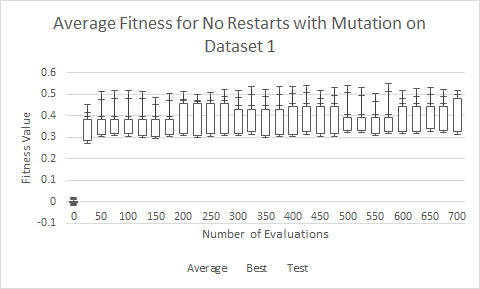
\includegraphics[width=0.8\textwidth]{res0adaptMuDS1}
\end{figure}
\begin{figure}[h]
	\centering
	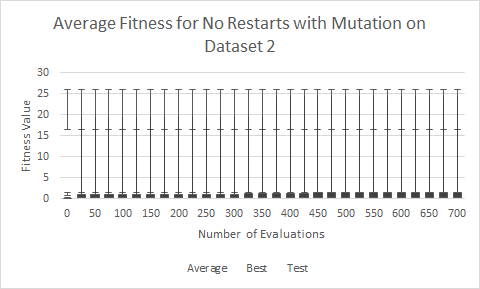
\includegraphics[width=0.8\textwidth]{res0adaptMuDS2}
\end{figure}
\newpage
\begin{figure}[h]
	\centering
	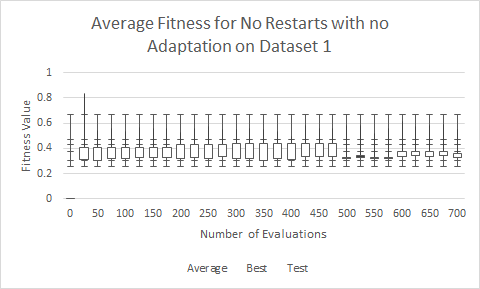
\includegraphics[width=0.8\textwidth]{res0adaptNoDS1}
\end{figure}
\begin{figure}[h]
	\centering
	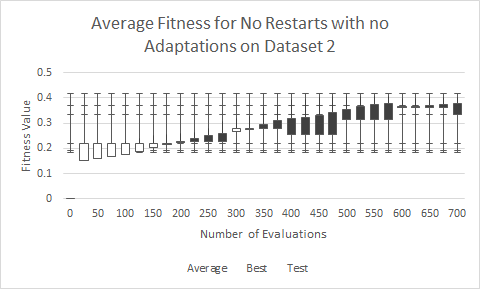
\includegraphics[width=0.8\textwidth]{res0adaptNoDS2}
\end{figure}
\newpage
\begin{figure}[h]
	\centering
	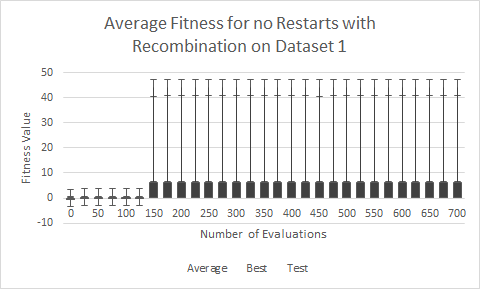
\includegraphics[width=0.8\textwidth]{res0adaptReDS1}
\end{figure}
\begin{figure}[h]
	\centering
	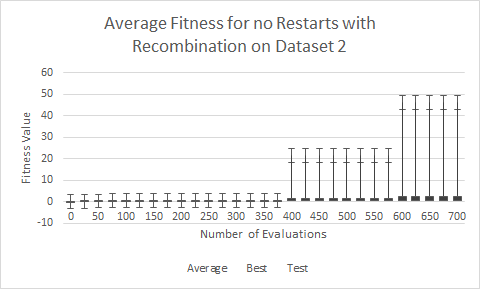
\includegraphics[width=0.8\textwidth]{res0adaptReDS2}
\end{figure}
\newpage
\begin{figure}[h]
	\centering
	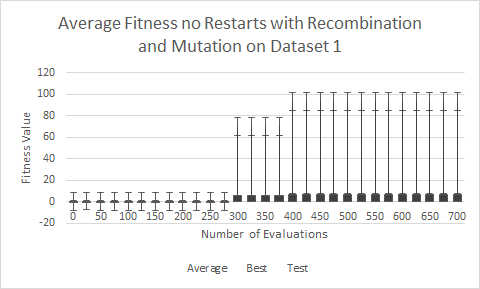
\includegraphics[width=0.8\textwidth]{res0adaptReMuDS1}
\end{figure}
\begin{figure}[h]
	\centering
	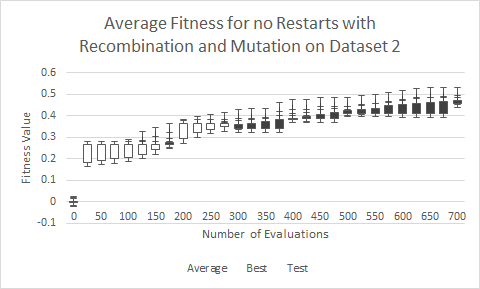
\includegraphics[width=0.8\textwidth]{res0adaptReMuDS2}
\end{figure}
\newpage
\begin{figure}[h]
	\centering
	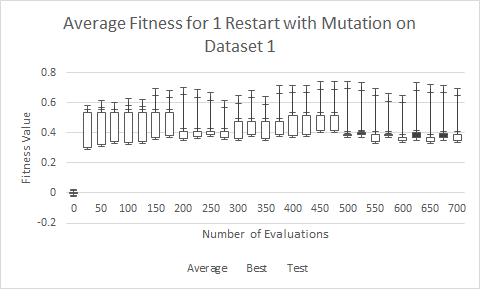
\includegraphics[width=0.8\textwidth]{res1adaptMuDS1}
\end{figure}
\begin{figure}[h]
	\centering
	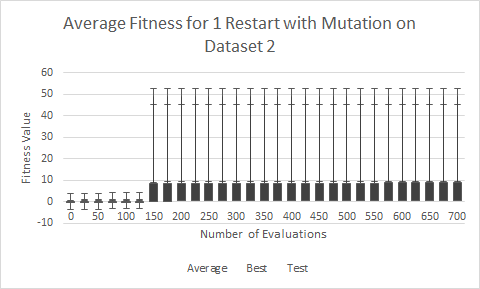
\includegraphics[width=0.8\textwidth]{res1adaptMuDS2}
\end{figure}
\newpage
\begin{figure}[h]
	\centering
	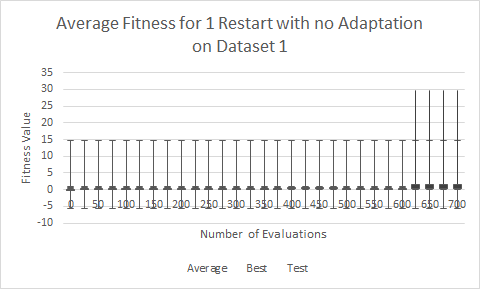
\includegraphics[width=0.8\textwidth]{res1adaptNoDS1}
\end{figure}
\begin{figure}[h]
	\centering
	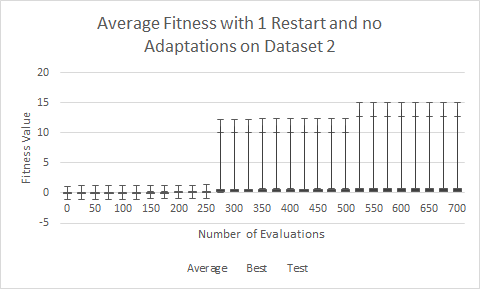
\includegraphics[width=0.8\textwidth]{res1adaptNoDS2}
\end{figure}
\newpage
\begin{figure}[h]
	\centering
	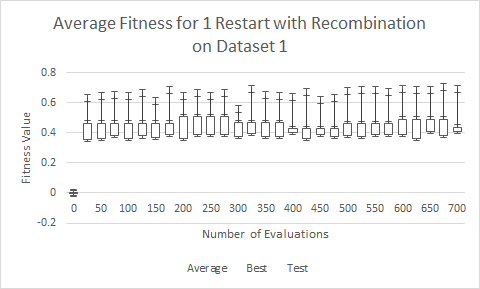
\includegraphics[width=0.8\textwidth]{res1adaptReDS1}
\end{figure}
\begin{figure}[h]
	\centering
	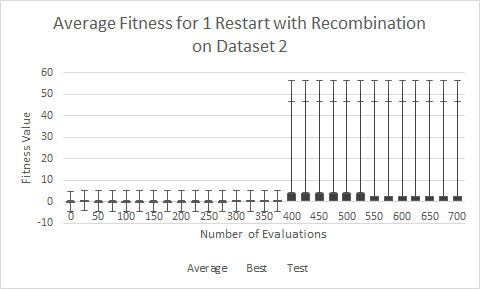
\includegraphics[width=0.8\textwidth]{res1adaptReDS2}
\end{figure}
\newpage
\begin{figure}[h]
	\centering
	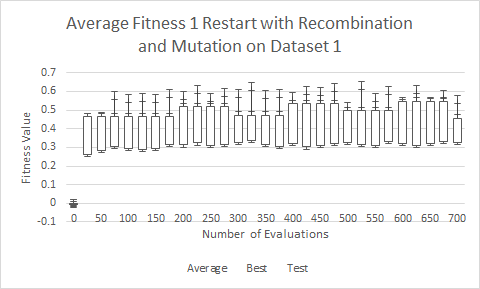
\includegraphics[width=0.8\textwidth]{res1adaptReMuDS1}
\end{figure}
\begin{figure}[h]
	\centering
	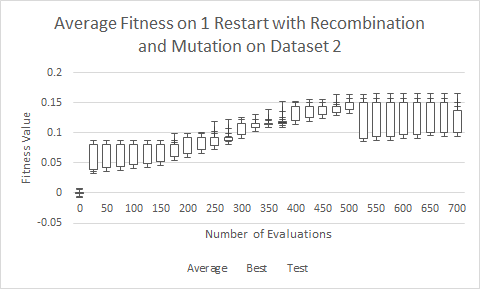
\includegraphics[width=0.8\textwidth]{res1adaptReMuDS2}
\end{figure}
\newpage
\begin{figure}[h]
	\centering
	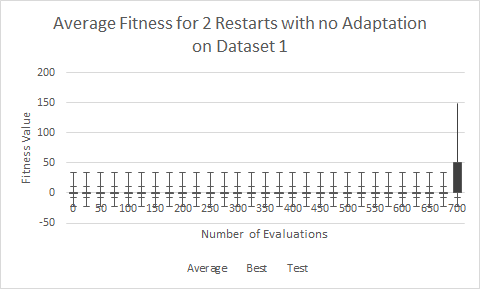
\includegraphics[width=0.8\textwidth]{res2adaptNoDS1}
\end{figure}
\newpage

\section{Experiment Comparisons}

\subsection{Control vs Mutation}
\subsubsection{Dataset 1}
\begin{figure}[h]
	\centering
	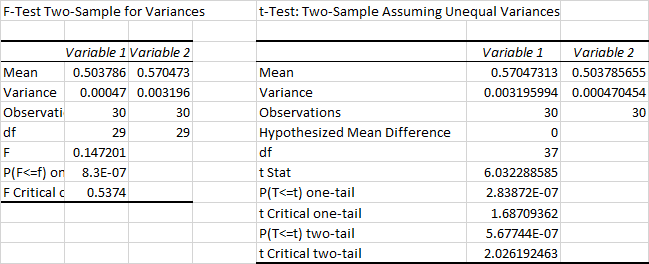
\includegraphics[width=0.8\textwidth]{DS1ControlvsMu}
\end{figure}
\subsubsection{Dataset 1}
\begin{figure}[h]
	\centering
	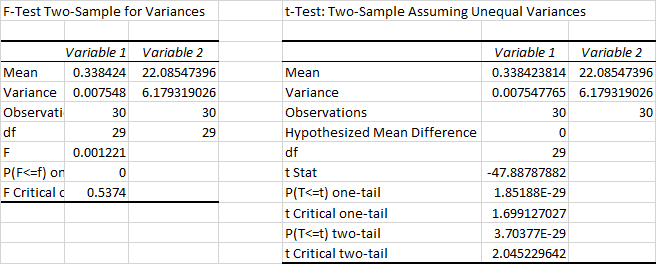
\includegraphics[width=0.8\textwidth]{DS2ControlvsMu}
\end{figure}
\begin{paragraph}
The F-Test was used to compare the two configurations. The results of the F-Test showed that
unequal variances should be assumed. After the t-test, it can be assumed that for dataset 1, the control was better with a 95% confidence.
It can also be assumed that for dataset 2, the control was worse with a 95% confidence.
\\
\end{paragraph}
\subsubsection{Dataset 2}
\begin{figure}[h]
	\centering
	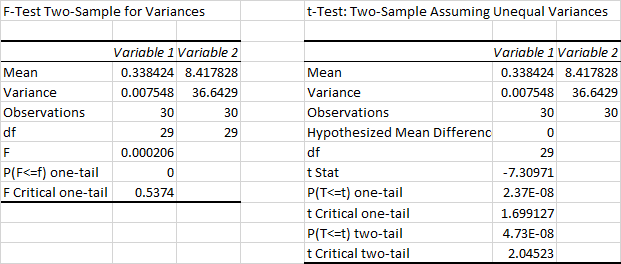
\includegraphics[width=0.8\textwidth]{DS2ControlvsR1}
\end{figure}
\subsubsection{Dataset 1}
\begin{figure}[h]
	\centering
	\includegraphics[width=0.8\textwidth]{DS2ControlvsR2}
\end{figure}
\begin{paragraph}
The F-Test was used to compare the two configurations. The results of the F-Test showed that
unequal variances should be assumed. After the t-test, it can be assumed that for dataset 1, the control was better with a 95% confidence.
It can also be assumed that for dataset 2, the control was worse with a 95% confidence.
\\
\end{paragraph}
\subsection{Control vs 1-Elitism Restarts}
\subsubsection{Dataset 1}
\begin{paragraph}
\\
\end{paragraph}
\subsubsection{Dataset 2}
\begin{paragraph}
\\
\end{paragraph}
\subsection{Control vs 2-Elitism Restarts}
\subsubsection{Dataset 1}
\begin{paragraph}
\\
\end{paragraph}
\subsubsection{Dataset 2}
\begin{paragraph}
\\
\end{paragraph}
\subsection{1-Elitism Restarts vs 2-Elitism Restarts}
\subsubsection{Dataset 1}
\begin{paragraph}
\\
\end{paragraph}
\subsubsection{Dataset 2}
\begin{paragraph}
\\
\end{paragraph}

\section{Bonus 1}

\subsection{Control vs Mutation with 1-Elitism Restarts}
\subsubsection{Dataset 1}
\begin{paragraph}
\\
\end{paragraph}
\subsubsection{Dataset 2}
\begin{paragraph}
\\
\end{paragraph}
\subsection{Mutation vs Mutation with 1-Elitism Restarts}
\subsubsection{Dataset 1}
\begin{paragraph}
\\
\end{paragraph}
\subsubsection{Dataset 2}
\begin{paragraph}
\\
\end{paragraph}
\subsection{1-Elitism Restarts vs Mutation with 1-Elitism Restarts}
\subsubsection{Dataset 1}
\begin{paragraph}
\\
\end{paragraph}
\subsubsection{Dataset 2}
\begin{paragraph}
\\
\end{paragraph}

\section{Bonus 2}

\subsection{Control vs Recombination}
\subsubsection{Dataset 1}
\begin{paragraph}
\\
\end{paragraph}
\subsubsection{Dataset 2}
\begin{paragraph}
\\
\end{paragraph}
\subsection{1-Elitism Restarts vs Recombination with Restarts}
\subsubsection{Dataset 1}
\begin{paragraph}
\\
\end{paragraph}
\subsubsection{Dataset 2}
\begin{paragraph}
\\
\end{paragraph}
\subsection{Control vs Recombination with Mutation}
\subsubsection{Dataset 1}
\begin{paragraph}
\\
\end{paragraph}
\subsubsection{Dataset 2}
\begin{paragraph}
\\
\end{paragraph}
\subsection{1-Elitism vs Recombination with Mutation}
\subsubsection{Dataset 1}
\begin{paragraph}
\\
\end{paragraph}
\subsubsection{Dataset 2}
\begin{paragraph}
\\
\end{paragraph}
\subsection{Mutation vs Recombination with Mutation}
\subsubsection{Dataset 1}
\begin{paragraph}
\\
\end{paragraph}
\subsubsection{Dataset 2}
\begin{paragraph}
\\
\end{paragraph}
\subsection{Mutation vs Recombination with Mutation and 1-Elitism Restarts}
\subsubsection{Dataset 1}
\begin{paragraph}
\\
\end{paragraph}
\subsubsection{Dataset 2}
\begin{paragraph}
\\
\end{paragraph}
\subsection{Recombination vs Recombination with Mutation}
\subsubsection{Dataset 1}
\begin{paragraph}
\\
\end{paragraph}
\subsubsection{Dataset 2}
\begin{paragraph}
\\
\end{paragraph}
\subsection{Recombination vs Recombination with Mutation and 1-Elitism Restarts}
\subsubsection{Dataset 1}
\begin{paragraph}
\\
\end{paragraph}
\subsubsection{Dataset 2}
\begin{paragraph}
\\
\end{paragraph}


\section{Conclusion}

\begin{flushleft}
In conclusion, in can be stated with 95\% confidence that both of the
evolutionary algorithms used are better than random search.
\end{flushleft}

\end{document}
